\documentclass[a4paper, oneside, final]{article}
\usepackage[T1]{fontenc}
\usepackage[utf8]{inputenc}
\usepackage[british]{babel}
\usepackage{amsmath}
\usepackage{amsthm}
\usepackage{verbatim}
\usepackage{listings}

\renewcommand{\britishhyphenmins}{22} 

\let\fref\undefined
\let\Fref\undefined

\usepackage{graphicx}
\usepackage{amssymb}

\setcounter{secnumdepth}{1} % Sæt overskriftsnummereringsdybde. Disable = -1.
\setlength{\parskip}{0.25in}

\pagestyle{plain}

\title{Topics in Programming Languages}

\begin{document}

\maketitle

\section{Abstract}

This report describes an implementation of the Par Monad in Eden which
is an extension of the Haskell programming language. To understand the
implementation a rudimentary understanding of Eden and the Par Monad is 
necessary hence the first two sections introduces these. 

\section{Eden}

Eden is a parallel functional programming language which extends
Haskell with constructs for the definition and instantiation of
parallel processes. Eden has been designed for distributed-memory
machines, i.e. clusters, this means that it is based on 
message-passing. This paradigm is very suitable for functional
programming and, as it turns out, very suitable for the Par Monad
as well. 

As mentioned Eden uses the process abstraction to provide parallelism.
The two main functions are \texttt{process} and \texttt{\#}. The
\texttt{process} functions turns a regular function into a parallel
processes and \texttt{\#} instantiates the parallel process with the
given argument and returns its result. \newline 

\begin{lstlisting}[language=Haskell, frame=tb, basicstyle=\footnotesize]
process :: ( Trans a , Trans b ) => (a -> b) -> Process a b
( # )   :: ( Trans a , Trans b ) => Process a b -> a -> b
\end{lstlisting}

These two functions are enough to write parallel programs. The example below shows a parallel implementation of the Fibonacci sequence \newline 

\begin{lstlisting}[language=Haskell, frame=tb, basicstyle=\footnotesize]
fib :: Int -> Int
fib 0 = 1
fib 1 = 1
fib n = process fib # (n-1) + process fib # (n-2)
\end{lstlisting}

Eden provides a variety of skeletons for parallel processing tasks
that  makes is faster to write parallel programs, however, they are
not used in our implementation so we won't cover them here.

Figure~\ref{edenstructure} shows the structure of Eden.

\begin{figure}[h]
  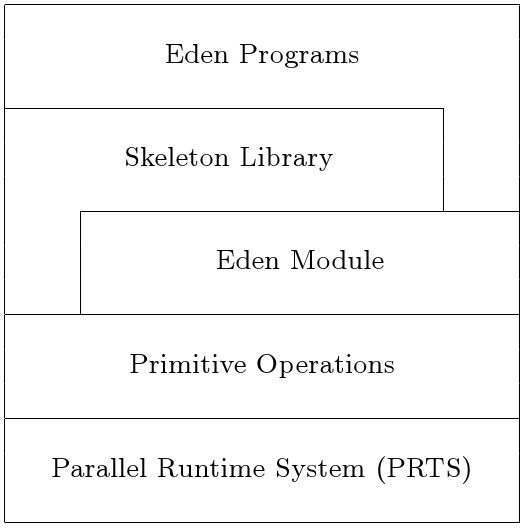
\includegraphics[width=5cm]{edenstructure.png}
  \label{edenstructure}
\end{figure}

\subsection{EDI}
\label{sub:edi}

TODO: Mads

\section{Par Monad}

The Par Monad was originally described in the paper ``A monad for deterministic parallelism''\cite{parmonad}. As the name suggests it is a monad for specifying pure parallel computations. It is especially well suited for dataflow networks. The purpose of this section is to make the reader comfortable with the Par Monad such that the next section will be understandable.

Given a computation in the Par Monad you can execute it concurrently with the current computation using the \texttt{fork} function. Computations in the \texttt{Par} monad can be extracted using the \texttt{runPar} function. \newline

\begin{lstlisting}[language=Haskell, frame=tb, basicstyle=\footnotesize]
fork :: Par () -> Par ()
runPar :: Par a -> a
\end{lstlisting}

The astute reader may notice that \texttt{fork} and \texttt{runPar} aren't very useful by themselves as you would never be able to read the values produced by the parallel computations. A way to communicate results from the child to the parent process is necessary; for this the Par monad uses a communication abstraction they call IVars. \texttt{IVar}'s also act as the entry point to the Par Monad. \newline

\begin{lstlisting}[language=Haskell, frame=tb, basicstyle=\footnotesize]
data IVar a 

new :: Par (IVar a)
get :: IVar a -> Par a
put :: NFData a => IVar a -> a -> Par ()
\end{lstlisting}

The \texttt{new} function creates a new IVar, \texttt{get} reads the value stored in the IVar and \texttt{put} writes a value to the IVar. If you invoke \texttt{get} on an empty \texttt{IVar} it will block until a value is stored in the \texttt{IVar}. Readers familiar with concurrent programming in Haskell may notice That this approach is very similar to the use of \texttt{MVar} with the main difference that IVars are write-once where \texttt{MVar}'s can be written multiple times.

These five functions are that is needed to write parallel programs using the Par Monad. The following listing shows a small example program taken from \texttt{Control.Monad.Par} on hackage\footnote{http://hackage.haskell.org/packages/archive/monad-par/0.1.0.1/doc/html/Control-Monad-Par.html} \newline

\begin{lstlisting}[language=Haskell, frame=tb, basicstyle=\footnotesize, numbers=left, numberstyle=\tiny]
runPar $ do
   [a,b,c,d] <- sequence [new,new,new,new]
   fork $ do x <- get a; put b (x+1)
   fork $ do x <- get a; put c (x+2)
   fork $ do x <- get b
             y <- get c 
             put d (x+y)
   fork $ do put a (3 :: Int)
   get d
\end{lstlisting}

On line 1 four \texttt{IVar}'s are created. Lines 2-8 creates tasks that read and write to different IVars in parallel. Line 9 reads the value stored in the IVar bound to d and as such this is the value returned by the entire program.The program is shown as a data-flow diagram below.

\begin{lstlisting}
                            a
                           / \  
                          b   c
                           \ /
                            d
\end{lstlisting}

This should be sufficient to understand the purpose and usage of the Par Monad.

\section{Implementing the Par Monad}

TODO: Mads

\section{Conclusion}

\bibliography{report}

\end{document}
